\documentclass[a4paper,11pt,headsepline]{report} % scrreprt würde auch gehen

\usepackage{titling}

%----------------- PDF CONFIG ----------------- %
\pdfinfo{    
     /Title     (Bachelorthesis ++Voller Name++ - HSRM WI - ++Titel++) 
     /Subject   (Bachelorhthesis ++Voller Name++)    
     /Author    (++Voller Name++) 
     /Keywords  (Bachelor,Bachelorthesis,HSRM)      
} 

\title{++Titel++}
\author{++Autor++}
\date{++AbgabeDatum++}



%----------------- PAKETE INKLUDIEREN ----------------- %

\usepackage[enable]{easy-todo} % Bietet eine art TODO Liste an; Zum bauen des abgabebereiten Dokumentes sollte die Option enable durch disable ersetzt werden!

\usepackage{geometry} % Packet für Seitenrandabständex und Einstellung für Seitenränder
\usepackage[ngerman]{babel} % deutsche Silbentrennung
\usepackage{blindtext} % Für den Beispieltext

\usepackage{booktabs} % entzerrt die Tabellenzeilen und bietet verschieden dicke Unterteilungslinien
\usepackage{longtable} % Tabellen können sich nicht über mehrere Seiten 
\usepackage{graphicx} % kann LaTeX Grafiken einbinden
%\usepackage{parskip}
\usepackage{xstring} % Für das FakeSmallCaps

\usepackage[utf8]{inputenc}
%\usepackage[applemac]{inputenc} % Umlaute unter Mac werden automatisch gesetzt
\usepackage[T1]{fontenc} % Zeichenencoding
\usepackage{lmodern} % bessere typographische Qualität 
\frenchspacing % Schaltet den zusätzlichen Zwischenraum ab; Wird mit ngerman-babel schon geladen
\usepackage{fix-cm}
\usepackage{color}
\usepackage[table]{xcolor}
\usepackage{enumitem}
\usepackage{url}
\usepackage{acronym}
\usepackage[ddmmyyyy,hhmmss]{datetime}
\renewcommand{\dateseparator}{.}

\usepackage{tabu} % Tabellen nutzen
\usepackage{multirow}
\usepackage{booktabs}
\usepackage{setspace} % to use \singlespacing\onehalfspacing\doublespacing
\usepackage{mathtools}

\usepackage{rotating} % For sidewayfigures
\usepackage{caption} % For centering the Captions if more than one Line
\captionsetup{justification=centering,margin=3em} % Set centering for captions as default

%----------------- SCHRFITEN ----------------- %
%\usepackage{bera} % Font package
%\usepackage{inconsolata} % MONOSPACE Font
%\usepackage{newcent}
\usepackage{charter} % modernere Serifen Font


\usepackage[nottoc]{tocbibind}

%----------------- BibLaTeX ----------------- %
\usepackage[
backend=bibtex,
style=alphabetic
]{biblatex}
\bibliography{literatur}

%----------------- EPIGRAPH ----------------- %
\usepackage{epigraph}
\setlength{\epigraphwidth}{0.7\textwidth} % Epigraph ist 70% der Textbreite breit
% Mache epigraph in Sans-Serif
\let\oldepigraph\epigraph % Gegen Rekursion
\renewcommand{\epigraph}[2]{\oldepigraph{\textsf{#1}}{\textsf{#2}}}

% für zweispaltige Inhalsverzeichnisse
% http://texblog.org/2013/08/14/tidy-and-compact-table-of-contents-with-multitoc/
% \usepackage[toc]{multitoc}
% \renewcommand*{\multicolumntoc}{2} % Spaltenanzahl; default 2
% \setlength{\columnseprule}{0.5pt} % Columnseperatingline


%----------------- LISTINGS ----------------- %
\usepackage{listings}

% LSTCOLORS
\definecolor{background}{HTML}{F1F1F1}

% Genrell Settings
\lstset{
  captionpos              = b,
  basicstyle              = \footnotesize\ttfamily,
%  backgroundcolor         = \color{background},
  numbers                 = left,
  numberstyle             = \scriptsize\color{background!70!black},
  stepnumber              = 1,
  numbersep               = 3ex,
  showstringspaces        = false,
  breaklines              = true,
  framesep                = 1ex,
  frame                   = l,%trb,
  framerule               = .35ex,
  xleftmargin             = 1.37ex,
%  frameround              = tttt,
  rulecolor               = \color{black},
  commentstyle            = \color{darkgray!80},
  escapeinside            = {<@[}{]@>}, % You can Escape inside the LST with <@[ ESCAPED_TEXT ]@>
  lineskip                = {-1.2pt},
  aboveskip               = {2em},
  belowskip               = {1em},
}

% PHP
\definecolor{dkgreen}{rgb}{0,.6,0}
\definecolor{dkblue}{rgb}{0,0,.6}
\definecolor{dkyellow}{cmyk}{0,0,.8,.3}
\definecolor{dkorange}{rgb}{1.0, 0.5, 0.0}

\lstset{
  language         = PHP,
  keywordstyle     = \color{dkblue},
  stringstyle      = \color{red},
  identifierstyle  = \color{dkgreen},
  emph             = [1]{php},
  emphstyle        = [1]\color{black},
  emph             = [2]{if,and,or,else,null,NULL},
  emphstyle        = [2]\color{dkorange},
  emph             = [3]{class,implements,namespace,public,private,protected,function,return,new,throw,try,catch,as,instanceof},
  emphstyle        = [3]\color{dkblue},
  morekeywords     = {class,implements,namespace,public,private,protected,function,return,new,throw,try,catch,as,instanceof},
}


% JSON  
\colorlet{punct}{red!60!black}
\definecolor{delim}{RGB}{20,105,176}
\colorlet{numb}{magenta!60!black}

\lstdefinelanguage{json}{
%  stringstyle      = \color{orange},
%  morestring       = [b]",
  literate         =
   *{0}{{{\color{numb}0}}}{1}
    {1}{{{\color{numb}1}}}{1}
    {2}{{{\color{numb}2}}}{1}
    {3}{{{\color{numb}3}}}{1}
    {4}{{{\color{numb}4}}}{1}
    {5}{{{\color{numb}5}}}{1}
    {6}{{{\color{numb}6}}}{1}
    {7}{{{\color{numb}7}}}{1}
    {8}{{{\color{numb}8}}}{1}
    {9}{{{\color{numb}9}}}{1}
    {:}{{{\color{punct}{:}}}}{1}
    {,}{{{\color{punct}{,}}}}{1}
    {\{}{{{\color{delim}{\{}}}}{1}
    {\}}{{{\color{delim}{\}}}}}{1}
    {[}{{{\color{delim}{[}}}}{1}
    {]}{{{\color{delim}{]}}}}{1}
    {"}{{{\color{red}{"}}}}{1}, % make " red
}

\lstdefinelanguage{yaml}{
  keywords        = {true,false,null},
  comment         = [l]{\#},
  morecomment     = [s]{/*}{*/},
  morestring      = [b]',
  morestring      = [b]",
}

%------------------Hyperref inkludieren -------------- %
% das Packet Hyperref erst nach allen anderen Inkludieren, damit auch Verweise
% auf Fußnoten korrekt geladen werden
\usepackage{hyperref} % verwandelt alle Kapitelüberschriften, Verweise aufs Literaturverzeichnis und andere Querverweise in PDF-Hyperlinks
%\usepackage{footnotebackref}    % Rück-Verweise von Fußnoten zu Verweis im Text (Wikipedia-Style)
%\usepackage{tablefootnote}         % für Fußnoten in Tabellen (dann \tablefootnote{Some Text} verwenden)

%----------------- FARBEN DEFINIEREN ----------------- %
% ~Hochschulfarben~
% Primary Colors
\definecolor{hsrmRed}{rgb}{0.882352941,0,0.098039216}
\definecolor{hsrmRedDark}{rgb}{0.588235294,0,0.058823529}
\definecolor{hsrmWarmGreyDark}{rgb}{0.274509804,0.254901961,0.235294118}
\definecolor{hsrmWarmGreyLight}{rgb}{0.666666667,0.647058824,0.62745098}

% Secondary Colors
\definecolor{hsrmSec1}{rgb}{0,0.588235294,0.509803922}
\definecolor{hsrmSec1Dark}{rgb}{0,0.392156863,0.31372549}
\definecolor{hsrmSec1Comp}{rgb}{0.294117647,0.745098039,0.882352941}
\definecolor{hsrmSec1CompDark}{rgb}{0.196078431,0.490196078,0.568627451}

\definecolor{hsrmSec2}{rgb}{0.607843137,0.764705882,0.156862745}
\definecolor{hsrmSec2Dark}{rgb}{0.411764706,0.490196078,0.098039216}
\definecolor{hsrmSec2Comp}{rgb}{0.254901961,0.156862745,0.509803922}
\definecolor{hsrmSec2CompDark}{rgb}{0.176470588,0.098039216,0.333333333}

\definecolor{hsrmSec3}{rgb}{0.509803922,0.078431373,0.31372549}
\definecolor{hsrmSec3Dark}{rgb}{0.338345865,0.058823529,0.196078431}
\definecolor{hsrmSec3Comp}{rgb}{1,0.509803922,0}
\definecolor{hsrmSec3CompDark}{rgb}{0.666666667,0.333333333,0}

% Custom Colors
\definecolor{gray}{gray}{0.95} % Listingsbackground
\colorlet{darkgray-light}{darkgray!90}

% Farbskala - um zB Prioritäten darzustellen
\definecolor{colorscale-green}{HTML}{DBFF33}
\definecolor{colorscale-yellow}{HTML}{FFF033}
\definecolor{colorscale-orange}{HTML}{FFBD33}
\definecolor{colorscale-dkorange}{HTML}{FF8A33}
\definecolor{colorscale-red}{HTML}{FF5733}
\definecolor{colorscale-gray}{gray}{.75}

%----------------- NEW Commands ----------------- %
% Eigener kurzer LoremIpsumDummyText
\newcommand{\sblindtext}{Dies hier ist ein Blindtext zum Testen von Textausgaben. Wer diesen Text liest, ist selbst schuld. Der Text gibt lediglich den Grauwert der Schrift an. Ist das wirklich so? Ist es gleichg\"{u}ltig, ob ich schreibe: ``Dies ist ein Blindtext'' oder ``Huardest gefburn''? Kjift $-$ mitnichten!}

% Define conclusionbox
\newcommand{\conclusionbox}[1]{\begin{center}\colorbox{darkgray!20}{\parbox{.9\textwidth}{#1}}\end{center}}

% Chapter Summary
\newcommand{\chaptersummary}[1]{\vspace{2em}\colorbox{darkgray-light}{\hspace{.03\textwidth}%
\parbox{.94\textwidth}{\vspace{.25em}%
\setlength{\parskip}{1.2ex}\bfseries\color{white}%
#1\vspace{1em}}%
\hspace{.03\textwidth}}%
\vspace{2em}}

% Fake Small Caps
\newcommand{\fakesmallcaps}[1]{\StrLeft{#1}{1} {\scriptsize\uppercase{\StrGobbleLeft{#1}{1}}}}

% Trenner
\newcommand{\trenner}{\centerline{\textcolor{risk-gray}{\rule{0.7\textwidth}{.4pt}}}}

% Table Midrule
\newcommand{\customcmidrule}[2]{\arrayrulecolor{#2}\cmidrule(l{1.5em} r{1.5em}){#1}\arrayrulecolor{black}}

% My Quote
\newenvironment{customquote}{\begin{quote}\raisebox{-.4\height}{{\Huge\color{darkgray-light} ''}}}{\end{quote}}



%----------------- LAYOUT SETZEN ----------------- %
\geometry{left=4.5cm, right=2cm, top=2.5cm, bottom=2.5cm}
\linespread {1.25}\selectfont %1.25 da er von Haus aus 1.2 ist und 1,25 * 1,2 = 1,5 isch
\setlength{\parindent}{0em} % im Deutschen Einrückung nicht üblich, leider
\setlength{\parskip}{1.2ex} % Abstand zum nächsten Absatz; evtl. KOMA verwenden?

%---------------- HEADER FOOTER ----------------------%
\usepackage{fancyhdr}
\pagestyle{fancy}
\newcommand{\phv}{\fontfamily{phv}\fontseries{m}\fontsize{9}{11}\selectfont}
%\addtolength{\headheight}{5ex} % damit man zwei Zeilen gut unterbringt
%\fancyhf{} % ClearFooter and Header
\fancyhead[LO,LE]{\small\selectfont\nouppercase\leftmark} % No uppercase and smaller fontsize
\fancyhead[RO,RE]{\small\selectfont\nouppercase\rightmark} % No uppercase and smaller fontsize
\lfoot{\phv \raisebox{-.24\height}{
\includegraphics[height=2.5ex]{media/logo_hsrm_single_bw}}\, ++Vorname++ \textsc{++Nachname++}} % \, ist ein kleiner Abstand
\cfoot{\thepage}




%-------##-------##-------##------- ANFANG INHALT -------##-------##-------##-------%
\begin{document}
\addtocontents{toc}{\protect\thispagestyle{empty}} % No Pagenumber on TOC Pages


\pagenumbering{roman} % Seitennummer

%----------------- DECKBLATT -----------------%
%----------------- KONFIGURATION ----------------- %
\pagestyle{empty} % enthalten keinerlei Kopf oder Fuß 

\newgeometry{left=4cm, right=2cm, top=1cm, bottom=1cm} % Mehr Platz oben und unten
%----------------- HS RM Logo ----------------- %
\begin{figure}[t]
	\flushright
	
\includegraphics[width=0.3\textwidth]{media/logo_hsrm}
\end{figure}

%----------------- INHALT ----------------- %

\begin{center}
Hochschule RheinMain \\
Fachbereich ++???++ \\
Studiengang ++???++

% Whitespace
\vspace{30 pt}

{\Large \textbf{Bachelor-Arbeit}} \\
zur Erlangung des akademischen Grades \\ 
Bachelor of Science - B.Sc.\todoi{Stimmt der Grad?}

% Whitespace
\vspace{50 pt}

\begin{spacing}{1.2}
\LARGE \textbf{\thetitle}
\end{spacing}
%
\end{center}

\vfill % Fills all the space, so the follwing stuff is floating down

%
\begin{small}
\begin{tabular}[h]{p{4cm}l l}
	vorgelegt von        & \textbf{++Vorname++ \textsc{++Nachname++}} \\ 
	                     & Matrikelnummer ++MatrNr++ \\
                	     & ++Straße / Hausnummer++ \\
	                     & ++PLZ Ort++ \\
	                     & \\
	am                   & \thedate \\
                	     & \\
	Referent:            & Prof. Dr. ++Vorname++ \textsc{++Nachname++}\\
	Korreferent:         & Prof. Dr. ++Vorname++ \textsc{++Nachname++}\\
	Betreuer extern:     & ++Titel++ ++Vorname++ \textsc{++Nachname++}\\
\end{tabular}
%
\vspace{15pt}
%
\begin{center}
	Durchgeführt bei der ++Firmenname++\\
	++Str / Nummer++, ++PLZ Ort++
\end{center}
\end{small}
%
\vspace{15pt}
%
\begin{center}
	\textcolor[gray]{0.4}{\tiny Kompiliert am \today ~um \currenttime ~- Erstellt mit \LaTeX}
\end{center}
%
\restoregeometry % Normales definiertes Layout

% Neue leere Seite erzeugen
\newpage
\thispagestyle{empty}
\quad \addtocounter{page}{-2} % Minus 2 um Deckblatt auch aus der Zählung zu nehmen
\newpage
 
%----------------- Formales -----------------%
%----------------- KONFIGURATION ----------------- %
\pagestyle{empty} % enthalten keinerlei Kopf oder Fuß


\chapter*{Formales} % (fold)
\label{cha:formales}
\textbf{Erklärung gem. ABPO, Ziff. 4.1.5.4 (3)}

\vspace{20pt}

Ich versichere, dass ich die Bachelor-Arbeit selbständig verfasst und keine anderen als die angegebenen Quellen und Hilfsmittel benutzt habe.

\vspace{20pt}

Ort, Datum\hfill Unterschrift Studierender

\vspace{25pt}

\noindent\makebox[5cm]{\hrulefill} \hfill \makebox[5cm]{\hrulefill}

\vspace{40pt}

\noindent\makebox[\linewidth]{\rule{\textwidth}{1pt}} % Horizontal Line

\vspace{40pt}

Hiermit erkläre ich mein Einverständnis mit den im Folgenden aufgeführten Verbreitungsformen dieser Bachelor-Arbeit:

\begin{center}
  \begin{tabular}{ | l | c | c | }
    \hline
    \textbf{Verbreitungsform}                                             & \textbf{ja} & \textbf{nein} \\ \hline
    Einstellung der Arbeit in die Hochschulbibliothek mit Datenträger     & X           &               \\ \hline
    Einstellung der Arbeit in die Hochschulbibliothek ohne Datenträger    & X           &               \\ \hline
	Veröffentlichung des Titels der Arbeit im Internet                    & X           &               \\ \hline
	Veröffentlichung der Arbeit im Internet                               & X           &               \\
    \hline
  \end{tabular}
\end{center}

\vspace{20pt}

Ort, Datum\hfill Unterschrift Studierender

\vspace{25pt}

\noindent\makebox[5cm]{\hrulefill} \hfill \makebox[5cm]{\hrulefill}

% ---------------- Sperrvermerk ------------- %
% Sperrvermerke sind zwar nicht erwünscht, kommen wenn aber hier herein
% \include{chapter/sperrvermerk}

%----------------- ABSTRACT ------------------%
%----------------- KONFIGURATION ----------------- %
\pagestyle{empty} % enthalten keinerlei Kopf oder Fuß


\chapter*{\centerline{Abstract}} % (fold)
\label{cha:abtract}

\section*{\centerline{Deutsch}}
\blindtext

\section*{\centerline{English}}
\blindtext

 
%----------------- VERZEICHNISSE -------------%
\tableofcontents % Inhaltverzeichnis

% Neue leere Seite erzeugen
\newpage
\thispagestyle{empty}
\quad \addtocounter{page}{-1}
\newpage

%--------##------- ANFANG CONTENT ------------##---------- %
\pagestyle{plain} % zurueck setzen von roemische seitenanzahl
\pagestyle{fancy}
\pagenumbering{arabic}

%----------------- KAPITEL : LIST OF TODOS ---------------%
\listoftodos

%----------------- KAPITEL : Einführung  ---------------- %
\chapter{Einführung}
\label{cha:einfuehrung}
\epigraph{Schlauer Spruch}{Verena \fakesmallcaps{Muster} - $\ast$1767 - \textit{Gelehrte / Schriftstellerin}}

%\chaptersummary{Mögliches Chapter Summary. Da aber Epigraph, hier kein Summary}

\blindtext




\section{Motivation}
\blindtext



\section{Ziel der Arbeit}
\sblindtext



\section{Aufbau der Arbeit}
\blindtext



\section{Umfeld}

\subsection{Deine Firma}
\blindtext


%----------------- KAPITEL : Grundlagen  ---------------- %
\chapter{Grundlagen}
\label{cha:grundlagen}

\chaptersummary{\sblindtext

Ja also darum gehts\dots}




\section{My Section}
\blindtext

\subsection{My Subsection}
\blindtext

\subsection{My Subsection 2}
\sblindtext

\subsubsection{My Sub Sub Section}
\sblindtext

\subsection{My Subsection 3}
\blindtext


%----------------- KAPITEL : Beispiele  ----------------- %
%----------------- KAPITEL : BEISPIELE  ----------------- %	
\chapter{Beispiele}
\label{cha:beispiele}
	Dieses Kapitel soll viele alltaegliche Beispiele\footnote{Fussnote} abdecken um einen {\LaTeX} Dokument zu setzen

		\section{Schriftarten}
		\label{sec:schriftarten} 
			\begin{itemize}
				\item Kursiv: \emph{Das ist ein Beispiel}
				\item Unterstreichen: \underline{Das ist ein Beispiel}
				\item Fettschrift: \textbf{Das ist ein Beispiel}
				\begin{itemize} 
					\item Kombination aus dreien: \underline{\textbf{\emph{Das ist ein Beispiel}}}						\end{itemize} 
				\item Serifen: \textsf{Das ist ein Beispiel}
				\item Schreibmaschinen Schrift: \texttt{Das ist ein Beispiel}
				\item Kleine Grossbuchstassen: \textsc{Das ist ein Beispiel}
				\item Ausfuehrungszeichen: ``Das ist ein Beispiel''
				\item asld
			\end{itemize}
			
		
			\subsection{Symbole}
				\begin{enumerate}
				\item Deutsche Umlaute: "A, "O, "U, "a, "o, "u, "s
				\item Sammlung von Sonderzeichen \url{http://de.wikibooks.org/wiki/LaTeX-Kompendium:_Sonderzeichen}
				\end{enumerate}
				

	\section{Abbildungen}
		Wie folgt bindet man Abbildungen ein:
		% Beispiel für Bildintegration
		\begin{figure}[htb]
		 \centering
		 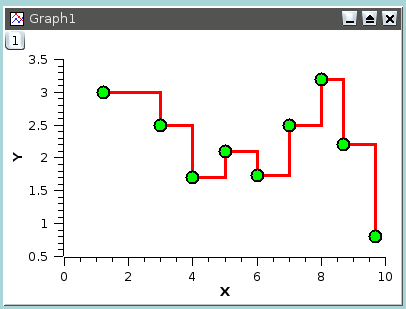
\includegraphics[width=0.4\textwidth,angle=0]{abb/beispiel}
 		\caption{Beispiel Bild; Quelle ist png}
		\label{fig:beispiel}
		\end{figure}
	
	\section{Tabellen}
			Lorem ipsum dolor sit amet, consetetur sadipscing elitr, sed diam nonumy eirmod tempor invidunt ut labore et dolore magna aliquyam erat, sed diam voluptua. At vero eos et accusam et justo duo dolores et ea rebum. Stet clita kasd gubergren.

		\begin{center}
			\begin{tabular}{lcrc} \toprule
			Stadium & Substratfreie Kontrolle  & \multicolumn{2}{c}{Probenansatz} \\\cmidrule(rl){3-4}
			 & Farbe & Farbe & Bewertung \\\midrule
			Alpha1 & farblos & braun & +++ \\
			Beta2 & farblos & farblos & - \\\bottomrule 
			 \end{tabular}
		 \end{center}
		 
		2. Beispiel \\
		\begin{table}[h]
		\centering	 
		 	\begin{tabular}{|l|l|c|}
			\hline
			\textsc{Rang} & \textsc{Name} & \textsc{Rating}\\
			\hline
			\hline
			1 & Garry Kasparov & 2817\\
			2 & Viswanathan Anand & 2774\\
			3 & Wladimir Kramnik & 2764\\
			\hline
			\end{tabular}
		\caption{Beispiel Beschriftung einer Tabelle}
		\label{tab:beispiel}
		\end{table}
		
		


	\section{Verweise}
		Hier werden Verweise auf verschiedene Elemente erstellt \cite{lin1973}
		\subsection{Pageref und Ref} 
			Diese Textstelle ist sehr interessant.\label{interessant} \\				
			Hier wird auf die Textstelle~\ref{interessant} verwiesen, \\
			die sich auf der Seite~\pageref{interessant} befindet.\\[20pt] 
			Verweis auf Listing \ref{lst:javaBsp} auf Seite \pageref{lst:javaBsp} \\
			Verweis auf Abbildung \ref{fig:beispiel} auf Seite \pageref{fig:beispiel} \\
			Verweis auf Tabelle \ref{tab:beispiel} auf Seite \pageref{tab:beispiel}
			
	\section{Listing}
		\lstset{language=java}
		\begin{lstlisting}[frame=hl, caption={Das Listing zeigt Java Quellcode} ,backgroundcolor=\color{gray}, label={lst:javaBsp}]
/* Java Hallo World Beispiel */

public class HelloWorld {
    public static void main(String[] args) {
        System.out.println("Hello, World");
    }
}
		\end{lstlisting} 
		
	
\nocite{wiki:xxx}

% Hier folgen nun die weiteren Kapitel

%----------------- KAPITEL : ???  ----------------------- %
% \include{chapter/???}

%----------------- KAPITEL : FAZIT  --------------------- %	
\chapter{Fazit und Ausblick}
\label{cha:fazit_ausblick}
\epigraph{Schlauer Spruch.}{Max \fakesmallcaps{Mustermann} - $\ast$2000BC - \textit{Naturwissenschaftler}}




\section{Fazit}
\label{sec:fazit}
\blindtext

\blindtext



\section{Ausblick}
\label{sec:ausblick}
\blindtext



\subsection{Entwicklungspotenziale}
\label{ssec:future-work}
Außerdem:

\begin{itemize}
	\item \dots
\end{itemize}




% Neue leere Seite erzeugen
\newpage
\thispagestyle{empty}
\quad %\addtocounter{page}{-1}
\newpage






%----------------- ANHANG (ROMAN) -------------%
\pagestyle{plain}
\pagenumbering{Roman}

%----------------- Danksagunggen -------------%
%----------------- KONFIGURATION ----------------- %
\thispagestyle{empty} % enthalten keinerlei Kopf oder Fuß

\newcommand{\dankespace}{\vspace{1.2em}}
\quad\hfill%
\begin{minipage}{.7\textwidth}
An dieser Stelle möchte ich mich bei allen bedanken, die mich in den letzten drei Monaten unterstützt haben.

\dankespace
Besonders möchte ich mich bei Herr Professor Dr. \textsc{++Nachname++} bedanken, der diese Arbeit betreut hat.
\sblindtext

\dankespace
\sblindtext

\dankespace
\blindtext

\vspace{7em}

\begin{footnotesize}\color{darkgray-light}
\begin{center}
Danke an \emph{(alphabetisch)}:\\
A \textsc{B} • C \textsc{D} • E \textsc{F} • G \textsc{H}
I \textsc{J} • K \textsc{L} • M \textsc{N} • O \textsc{P}
\end{center}
\end{footnotesize}
\end{minipage}%
\hfill\quad



%----------------- CD Infos -------------%
\chapter*{CD-Informationen}
\addcontentsline{toc}{chapter}{CD-Informationen}
Informationen zu der beigefügten CD. Der Datenträger ist an der inneren hinteren Einbandseite zu finden.

\section*{Inhalt}
\begin{itemize}
	\item Bachelorarbeit als PDF
	\item \dots
\end{itemize}



%----------------- VERZEICHNISSE II ---------------------- %

% ---------------- Abkürzungsverzeichnis ---- %
\chapter*{Abkürzungsverzeichnis}
\addcontentsline{toc}{chapter}{Abkürzungsverzeichnis}
\begin{acronym}[LängsteAbkürzungHierRein]
	\acro{zB}{zum Beispiel}
\end{acronym}
\clearpage

% ---------------- Gloassar ---------------- %
\chapter*{Glossar}
\label{cha:glossar}
\addcontentsline{toc}{chapter}{Glossar}
% I could use https://en.wikibooks.org/wiki/LaTeX/Glossary instead

\begin{description}[leftmargin=3cm,style=nextline]
	\item[Beispiel]
		\sblindtext
\end{description}
\clearpage

% ----- Abbildungen ----- %
%\addcontentsline{toc}{section}{Abbildungsverzeichnis} % falls in Inhalsverzeichnis
\listoffigures
\clearpage

% ----- Tabellen----- %
% \addcontentsline{toc}{section}{Tabellenverzeichnis}  % falls in Inhalsverzeichnis
% \fancyhead[L]{Abbildungsverzeichnis / Abkürzungsverzeichnis} %Kopfzeile links
\listoftables
\clearpage

% ----- Listings ----- %
% Listingverzeichnis soll im Inhaltsverzeichnis auftauchen
% \fancyhead[L]{Abbildungs- / Tabellen- / Listingverzeichnis} %Kopfzeile links
\renewcommand{\lstlistlistingname}{Listingverzeichnis}
\lstlistoflistings
\addcontentsline{toc}{chapter}{Listingverzeichnis}
\clearpage

%----------------- Literaturverzeichnnis ------------------%
\printbibliography
\addcontentsline{toc}{chapter}{Literatur}

\end{document}
